\section{光的直线传播}\label{sec:1-1}

光是从一些物体发出来的。例如太阳、电灯、蜡烛的火焰等都能够发光。
这些能发光的物体叫做\textbf{光源}。光源发出来的光是怎样向周围传播的呢?

打扫房间的时候,如果有太阳光穿过窗户射进屋子里,照着飘浮的灰尘,会看到光通过的路线是直的。
穿过云隙的太阳光,黑夜里手电筒的光,通过的路线也是直的。这些现象表明,光在空气里是沿直线传播的。

光不仅能在空气里传播,而且还可以在水、玻璃等透明物质里传播。
实验表明,光在任何一种透明物质里传播的路线都是直的。
但是,如果光从一种物质(例如空气)进入另一种物质(例如水或玻璃),它的传播方向通常会改变。
因此,应该说:

\textbf{光在同一种物质里传播的路线是直的}。

通常所说的光线,指的是光通过的路线。所以,上面的结论可以这样说:
\CJKunderwave{在同一种物质里,光线是直的}。

光从光源发出来,照射到物体,需要时间吗?
很早以前,人们认为光的传播是不需要时间的。
根据日常经验,这种看法似乎是对的。
当你打开电灯的时候,整个房间几乎同时都被照亮了。
你觉察不出离电灯近的地方比远的地方会早亮一些。

\begin{enhancedline}[1ex]
但是,实际上光是以一定的速度传播的。
只是由于光的速度非常大,通过不太长的距离需要的时间非常短,因此不易觉察到。
直到十七世纪后半期,人们才第一次测出了光的速度。
现在我们知道,光在真空中的速度是 $3 \times 10^5 \qmmm$。
这个速度相当于一秒钟绕地球赤道七圈半。
光在真空中的速度最大,在空气中的速度跟在真空中的差不多。
因此通常认为光在空气中的速度也是 $3 \times 10^5 \qmmm$。
光在水里的速度大约是空气里的 $\dfrac{3}{4}$。
在玻璃里的速度比在水里的还小。
\end{enhancedline}

光比声音的传播快得多。声音在空气里的速度是 $340\mmm$。
现在你就会明白,虽然闪电和雷声是同时发生的,但是我们却先看见闪电后听到雷声。

\section*{阅读材料}

在我国古书《墨经》中,记载了当时墨家学派的代表人物墨瞿〈约公元前468 ~ 公元前376 )
和他的学生做的世界上最早的小孔成像实验。

\begin{figure}[htbp]
    \centering
    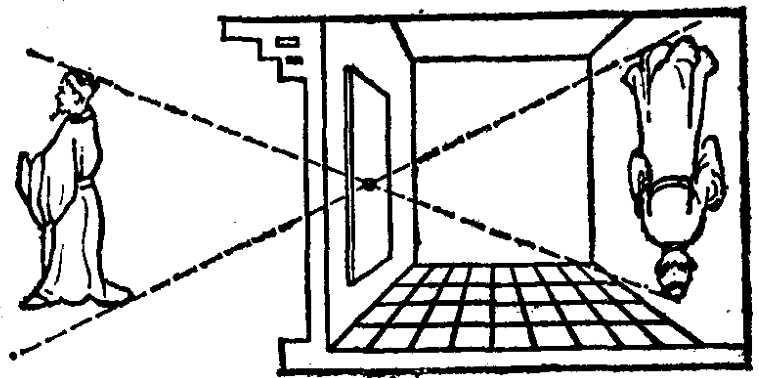
\includegraphics[width=0.7\textwidth]{../pic/czwl2-ch1-1}
    \caption{小孔成像}\label{fig:1-1}
\end{figure}

在一间黑暗的小屋朝阳的墙上开一个小孔。在屋外,小孔的前方站着一个人。
这时屋里相对的墙上就出现了一个倒立的人像〈图 \ref{fig:1-1})。
为什么会出现这奇怪的现象呢?书中解释说,这是因为光象射箭一样,是直线行进的。
从人体上部射来的光,通过小孔,投射在下边;
从人体下部射来的光,通过小孔,投射在上边,这就形成了倒立的像。
并且还指出,人的位置离墙壁由远而近,它的像也由小变大,倒立在墙上。

这个实验到现在已有二千四五百年。
《墨经》在解释小孔成像时明确提出了光的传播路线是直的。
这是世界上关于光的直线传播的最早记载。


\lianxi

(1) 在硬纸上穿一个小洞,通过小洞向外看时,为什么眼睛离小洞越近,看到的范围就越大?

(2) 如图 \ref{fig:1-2} 所示,在灯光下靠近墙的地方,用两只手做出各种姿态,你会看到,
墙上的手影形成马、狗、鸭等的生动形象。自己实际做做,并且想想看,
什么样的物体后面有影子?光源发出的光为什么射不到影子里?

\begin{figure}[htbp]
    \centering
    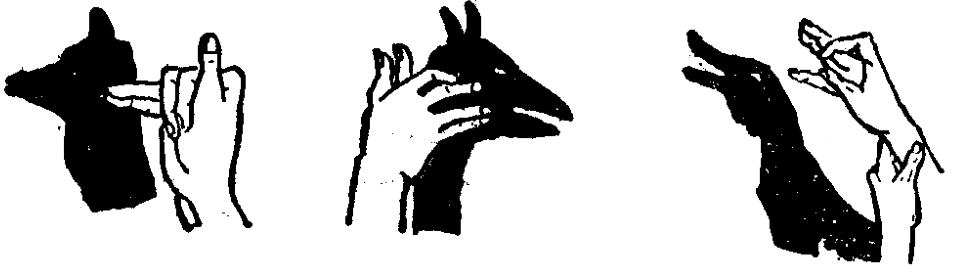
\includegraphics[width=0.7\textwidth]{../pic/czwl2-ch1-2}
    \caption{}\label{fig:1-2}
\end{figure}


(3) 在太阳光的照射下,人在地面上的影子为什么早晚长,中午短?画图来帮助说明。

(4) 天文学上常用光年〈就是光在一年内通过的距离)来做长度的单位,1 光年是多少千米?
织女星离地球约 27 光年,织女星离地球有多少千米?

(5) 有一位在北京某剧场里观看演出的观众坐在离演奏者 30 米远处,
另一位在上海的观众在自己家里电视机前看该剧场的电视转播演出,
北京与上海相距 1460 千米。问哪一位观众先听到演奏声?
电视是靠无线电波来转播的,而无线电波与光的传播速度相等。


\section*{小实验}

\begin{wrapfigure}[7]{r}{6cm}
    \centering
    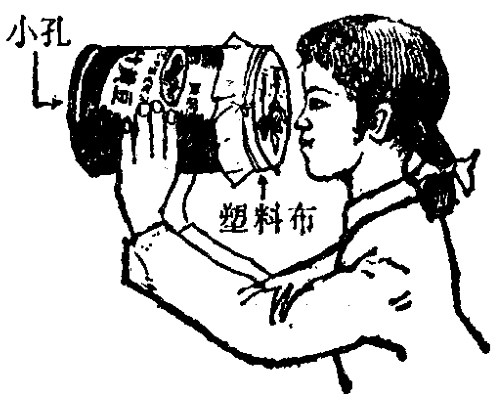
\includegraphics[width=4cm]{../pic/czwl2-ch1-3}
    \caption{}\label{fig:1-3}
\end{wrapfigure}

你可以自己做小孔成像的实验。找一个空罐头筒(或一个方纸盒)。
在筒底的中心用小铁钉开一个小孔(直径 1 毫米到 3 毫米),
在开口端蒙上一块半透明的塑料布(或纸)。
让罐头筒上的小孔对着房间外边明亮的景物,在你的头和罐头筒上面蒙上一件厚的深颜色衣服。
你在塑料布上就会看到一幅彩色的图像(图 \ref{fig:1-3}),只可惜是倒立的。

利用这样的装置,装上底片就可以拍摄出清晰的照片来。


